\documentclass{../ucll-slides}
\usepackage{pxfonts}
\usepackage{tikz}
\usepackage{calc}
\usepackage{../ucll-code}


\usetikzlibrary{calc,shadows,tikzmark}

\coursename{Distributed Applications}
\title{Linked Lists}

\pgfkeys{
  /custom/.cd,
  width/.initial=1cm,
  height/.initial=1cm,
  position/.initial={0,0},
  size/.style={width=#1,height=#1},
  value/.initial={},
  value font/.initial={\ttfamily}
}

\newcommand{\llnode}[1][1]{
    {
        \pgfkeys{/custom/.cd,#1}
        \pgfkeys{/custom/width/.get=\llnodewidth}
        \pgfkeys{/custom/height/.get=\llnodeheight}
        \pgfkeys{/custom/position/.get=\llnodeposition}
        \pgfkeys{/custom/value/.get=\llnodevalue}
        \pgfkeys{/custom/value font/.get=\llnodevaluefont}
        \draw[thick] (\llnodeposition) rectangle ++(\llnodewidth,\llnodeheight);
        \draw[thick] ($ (\llnodeposition) + (\llnodewidth,0) $) rectangle ++(\llnodewidth,\llnodeheight);
        \node[font=\llnodevaluefont] at ($ (\llnodeposition) + (\llnodewidth / 2,\llnodeheight / 2) $) {\llnodevalue};
    }
}

\begin{document}

\maketitle

% \input{aux-overview}
% \section{Memory Layout}

\frame{\tableofcontents[currentsubsection]}

\begin{frame}
    \frametitle{Arrays}
    \begin{center}
        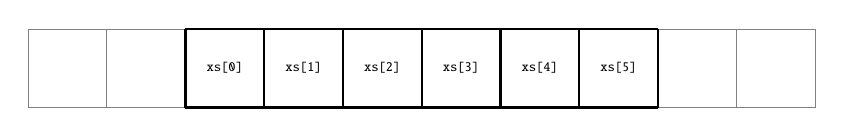
\begin{tikzpicture}
            \draw[help lines] (-2,0) grid (8,1);
            \draw[thick] (0,0) grid (6,1);
            \foreach \x in {0,...,5} {
                \node[font=\tiny] at ($ (\x,0.5) + (0.5,0) $) { \texttt{xs[\x]} };
            }
        \end{tikzpicture}
    \end{center}
    \vskip4mm
    \begin{itemize}
        \item One piece of contiguous memory
    \end{itemize}
\end{frame}

\begin{frame}
    \frametitle{Arrays}
    \code[language=c++14]{array.cpp}
\end{frame}

\begin{frame}
    \frametitle{Linked Lists}
    \begin{center}
        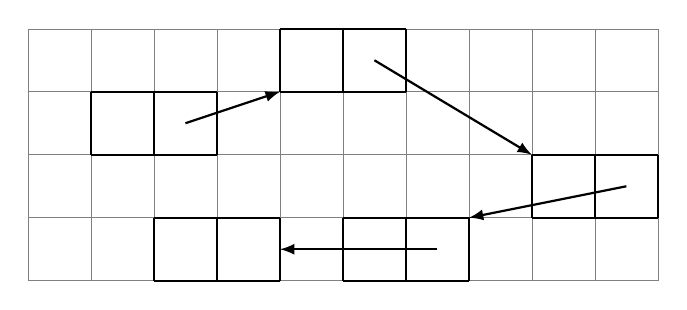
\begin{tikzpicture}[link/.style={thick,-latex},scale=0.8,transform shape]
            \draw[help lines] (0,0) grid (10,4);
            \draw[thick] (1,2) grid ++(2,1);
            \draw[thick] (4,3) grid ++(2,1);
            \draw[thick] (5,0) grid ++(2,1);
            \draw[thick] (2,0) grid ++(2,1);
            \draw[thick] (8,1) grid ++(2,1);

            \draw[link] (2.5,2.5) -- (4,3);
            \draw[link] (5.5,3.5) -- (8,2);
            \draw[link] (9.5,1.5) -- (7,1);
            \draw[link] (6.5,0.5) -- (4,0.5);
        \end{tikzpicture}
    \end{center}
    \vskip4mm
    \begin{itemize}
        \item List consists of series of nodes
        \item Each node has two fields
              \begin{itemize}
                \item Item
                \item Reference to next node
              \end{itemize}
        \item Nodes spread across memory
    \end{itemize}
\end{frame}

\begin{frame}
    \frametitle{Linked Lists in Code}
    \code[language=csharp]{LinkedList.cs}
\end{frame}

\begin{frame}
    \frametitle{Creating a Linked List}
    \begin{center}
        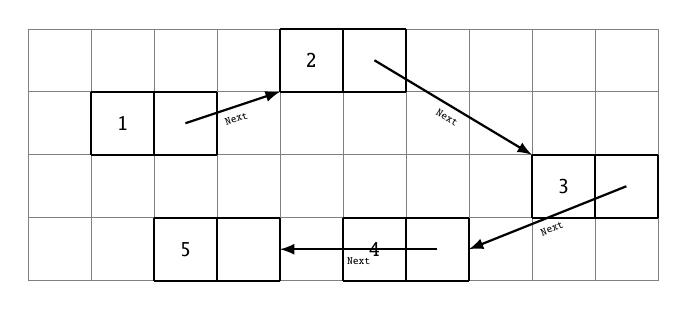
\begin{tikzpicture}[link/.style={thick,-latex},scale=0.8,transform shape]
            \draw[help lines] (0,0) grid (10,4);
            \draw[thick] (1,2) grid ++(2,1);
            \draw[thick] (4,3) grid ++(2,1);
            \draw[thick] (5,0) grid ++(2,1);
            \draw[thick] (2,0) grid ++(2,1);
            \draw[thick] (8,1) grid ++(2,1);

            \draw[link] (2.5,2.5) -- (4,3) node[midway,font=\tiny\ttfamily,sloped,below]{Next};
            \draw[link] (5.5,3.5) -- (8,2) node[midway,font=\tiny\ttfamily,sloped,below]{Next};
            \draw[link] (9.5,1.5) -- (7,0.5) node[midway,font=\tiny\ttfamily,sloped,below]{Next};
            \draw[link] (6.5,0.5) -- (4,0.5) node[midway,font=\tiny\ttfamily,sloped,below]{Next};

            \node[font=\ttfamily] at (1.5,2.5) {1};
            \node[font=\ttfamily] at (4.5,3.5) {2};
            \node[font=\ttfamily] at (8.5,1.5) {3};
            \node[font=\ttfamily] at (5.5,0.5) {4};
            \node[font=\ttfamily] at (2.5,0.5) {5};
        \end{tikzpicture}
    \end{center}
    \vskip4mm
    \code[language=csharp]{LinkedListCreation.cs}
\end{frame}
% \section{Determining Length}

\frame{\tableofcontents[currentsubsection]}

\begin{frame}
    \frametitle{Length of Array}
    \begin{itemize}
        \item Array must keep track of Length
        \item Computing length is immediate ($O(1)$)
    \end{itemize}
\end{frame}

\begin{frame}
    \frametitle{Length of Linked List}
    \begin{center}
        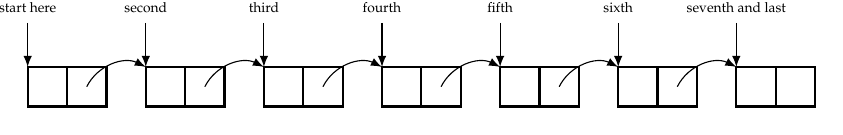
\begin{tikzpicture}[link/.style={thick,-latex}]
            \path[use as bounding box] (0,0) rectangle (10,1);

            \foreach[count=\i] \x in {0,1.5,...,10} {
                \coordinate (p\i) at (\x,0);
                \draw[thick] (p\i) rectangle ++(0.5,0.5);
                \draw[thick] ($ (p\i) + (0.5,0) $) rectangle ++(0.5,0.5);
            }

            \foreach[count=\i] \x in {0,1.5,...,8} {
                \draw[-latex] ($ (p\i) + (0.75,0.25) $) to[bend left=45] ++(0.75,0.251);
            }

            \foreach \i/\label in {1/{start here},2/{second},3/{third},4/{fourth},5/{fifth},6/{sixth},7/{seventh and last}} {
                \only<\i>{
                    \node[font=\tiny] (label) at ($ (p\i) + (0,1.25) $) {\label};
                    \draw[-latex] (label.south) -- ($ (p\i) + (0,.5) $);
                }
            }
        \end{tikzpicture}
    \end{center}
    \vskip4mm
    \structure{Algorithm}
    \begin{itemize}
        \item Follow nodes until we find \texttt{null}
        \item Count number of jumps necessary
        \item Takes longer for longer lists
    \end{itemize}
\end{frame}
% \begin{frame}
    \frametitle{Indexing Array}
    \begin{center}
        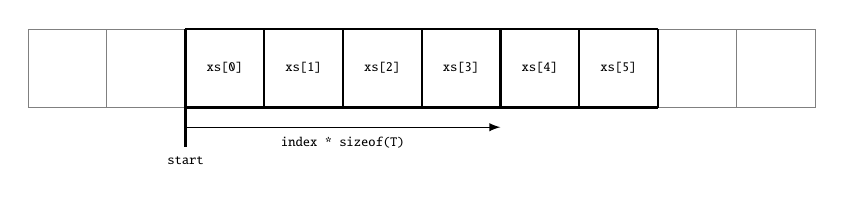
\begin{tikzpicture}
            \draw[help lines] (-2,0) grid (8,1);
            \draw[thick] (0,0) grid (6,1);
            \foreach \x in {0,...,5} {
                \node[font=\tiny] at ($ (\x,0.5) + (0.5,0) $) { \texttt{xs[\x]} };
            }
            \draw[thick] (0,0) -- ++(0,-0.5);
            \node[anchor=north,font=\ttfamily\tiny] at (0,-0.5) {start};
            \draw[|-latex] (0,-.25) -- ++(4,0) node[midway,below,font=\tiny\ttfamily] {index * sizeof(T)};
        \end{tikzpicture}
    \end{center}
    \vskip4mm
    \structure{Algorithm}
    \begin{itemize}
        \item Memory location can be computed in a single step
        \item \texttt{location = start + index * sizeof(T)}
        \item Direct CPU support: only 1 instruction required
        \item Explains zero-indexing
        \item $O(1)$
    \end{itemize}
\end{frame}

\begin{frame}
    \frametitle{Indexing Linked List}
    \begin{center}
        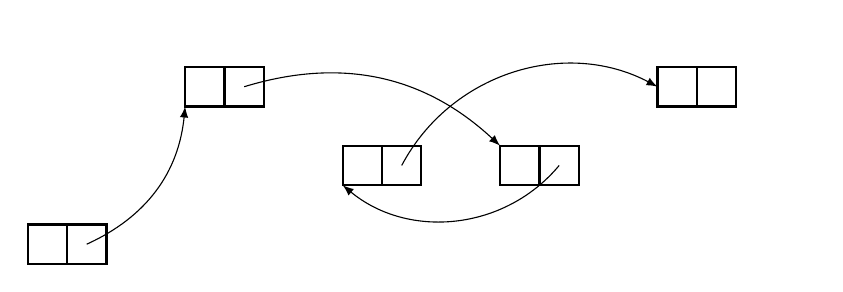
\begin{tikzpicture}[link/.style={thick,-latex}]
            \path[use as bounding box] (0,0) rectangle (10,3);
            \coordinate (p1) at (0,0);
            \coordinate (p2) at (2,2);
            \coordinate (p4) at (4,1);
            \coordinate (p3) at (6,1);
            \coordinate (p5) at (8,2);

            \foreach \i in {1,...,5} {
                \draw[thick] (p\i) rectangle ++(0.5,0.5);
                \draw[thick] ($ (p\i) + (0.5,0) $) rectangle ++(0.5,0.5);
            }

            \draw[-latex] ($ (p1) + (0.75,0.25) $) to[bend right=30] (p2);
            \draw[-latex] ($ (p2) + (0.75,0.25) $) to[bend left=30] ($ (p3) + (0,0.5) $);
            \draw[-latex] ($ (p3) + (0.75,0.25) $) to[bend left=45] ($ (p4) + (0,0) $);
            \draw[-latex] ($ (p4) + (0.75,0.25) $) to[bend left=45] ($ (p5) + (0,0.25) $);
        \end{tikzpicture}
    \end{center}
    \vskip4mm
    \structure{Algorithm}
    \begin{itemize}
        \item Nodes are scattered across memory
        \item Follow \texttt{Next} until \texttt{Next == null}
        \item Finding \texttt{n}th element takes \texttt{n} jumps
        \item $O(n)$
    \end{itemize}
\end{frame}

% \input{aux-update}
% \input{aux-prepend}
\input{aux-concatenate}


% \begin{frame}
%     \frametitle{Comparison}
%     \begin{center}
%         \begin{tabular}{lcc}
%             & \textbf{Array} & \textbf{Linked List} \\
%             \midrule
%             Length & $O(1)$ & $O(n)$ \\
%             Indexing & $O(1)$ & $O(n)$ \\
%             Add to front & $O(n)$ & $O(1)$ \\
%             Add to end & $O(n)$ & $O(n)$ \\
%             Concatenation & $O(n_1+n_2)$ & $O(n_1)$ \\
%             \bottomrule
%         \end{tabular}
%     \end{center}
% \end{frame}

\end{document}

%%% Local Variables:
%%% mode: latex
%%% TeX-master: t
%%% End:
